\setcounter{page}{1}


\section{Introducción}
    El diseño y la administración de redes de computadoras es componente esencial para garantizar la eficiencia, seguridad y escalabilidad de las infraestructuras tecnológicas que sustentan diversas organizaciones. En este contexto, el uso de Redes de Área Local Virtual (VLAN) ha surgido como una solución eficaz para optimizar la segmentación de redes, permitiendo no solo mejorar la administración de recursos, sino también establecer políticas de acceso y comunicación más robustas dentro de las organizaciones.

    Este documento realizaremos una práctica orientada a la implementación de VLANs utilizando el simulador Cisco Packet Tracer, herramienta que permite diseñar, configurar y evaluar redes de manera segura y controlada. En esta práctica, se abordan conceptos fundamentales relacionados con la segmentación de redes, la asignación de direcciones IP y el establecimiento de comunicaciones específicas entre dispositivos.

    En el trabajo se detallan tanto los objetivos como los pasos específicos llevados a cabo para configurar VLAN's que simulan entornos empresariales reales. Desde la definición de las configuraciones iniciales en los switches hasta la asignación de dispositivos a las respectivas VLAN's, cada etapa del proceso busca consolidar habilidades prácticas en el diseño de redes eficientes. Asimismo, se evalúa la correcta funcionalidad de la segmentación de red mediante pruebas que comprueban la conectividad entre los equipos.

    Con este ejercicio, se pretende no solo reforzar los conocimientos teóricos adquiridos en el aula, sino también brindar una experiencia práctica que permita comprender de manera integral cómo implementar tecnologías de red avanzadas. A través de este enfoque, se fomenta una mayor capacidad para enfrentar desafíos reales en la administración y diseño de redes modernas.

\section{Objetivos}
    \begin{itemize}
        \item Implementar VLAN de acceso.
        \item Identicar IP's con clase.
    \end{itemize}

\section{Desarrollo del Trabajo}

    \begin{table}[H]
        \begin{center}
            \begin{tabular}{ c | c | c | c }
                \textbf{VLAN} & \textbf{Nombre} & \textbf{Puertos} & \textbf{Red}\\ \hline
                2 & ELECTRONICA & 2,4,6,8 & 1.0.0.0/8\\
                4 & SISTEMAS & 10,12,14,16 & 10.0.0.0/8\\
                6 & CIVIL & 1,3,5,7 & 172.16.0.0/16\\
                8 & ELECTRICA & 9,11,13,15 & 192.168.6.0/24\\
            \end{tabular}
            \caption{VLAN's}
            \label{tab:VLANs}
            \end{center}
    \end{table}

    \subsection{Configuración de las VLAN's en Cisco Packet Tracer PC1}
        Para comenzar a configurar, en el simulador agregamos un Switch, 4 servidores y 12 PC's. Posteriormente, procedemos a conectar los dispositivos de acuerdo al puerto asignado en la tabla~\ref{tab:VLANs}, según la VLAN a la que se desea asignar. En la figura~\ref{fig:cisco} se muestra la configuración en el simulador Cisco Packet Tracer.

        \begin{figure}[H]
            \centering
            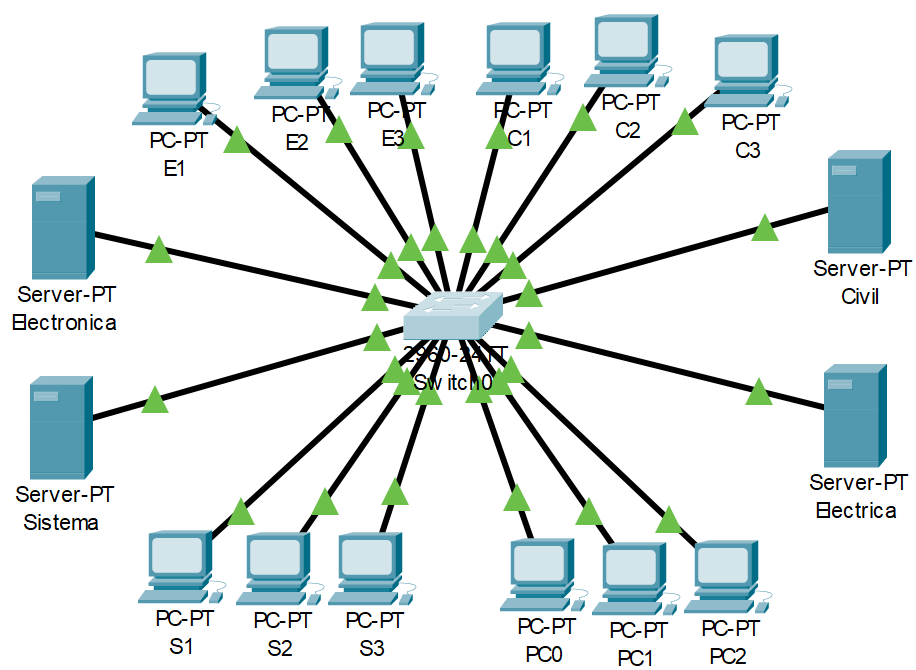
\includegraphics[width=0.6\textwidth]{img/cisco.png}
            \caption{Configuración en el simulador Cisco Packet Tracer}
            \label{fig:cisco}
        \end{figure}

        Para configurar la VLAN 2 en el switch y asignar los puertos correspondientes al departamento de Electrónica, es necesario acceder a la terminal del switch y ejecutar los siguientes comandos:

        \begin{lstlisting}[language=bash, caption={Creación y configuración de la VLAN 2},label={lst:cisco_vlan2}]
            Switch(config)# vlan 2
            Switch(config-vlan)# name ELECTRONICA
            Switch(config)# interface range fa0/2, fa0/4, fa0/6, fa0/8
            Switch(config-if-range)# switchport mode access
            Switch(config-if-range)# switchport access vlan 2
        \end{lstlisting}

        Para configurar la VLAN 4 en el switch y asignar los puertos correspondientes al departamento de Sistemas, es necesario acceder a la terminal del switch y ejecutar los siguientes comandos:

        \begin{lstlisting}[language=bash, caption={Creación y configuración de la VLAN 4},label={lst:cisco_vlan4}]
            Switch(config)# vlan 4
            Switch(config-vlan)# name SISTEMAS
            Switch(config)# interface range fa0/10, fa0/12, fa0/14, fa0/16
            Switch(config-if-range)# switchport mode access
            Switch(config-if-range)# switchport access vlan 4
        \end{lstlisting}

        Para configurar la VLAN 6 en el switch y asignar los puertos correspondientes al departamento de Civil, es necesario acceder a la terminal del switch y ejecutar los siguientes comandos:

        \begin{lstlisting}[language=bash, caption={Creación y configuración de la VLAN 6},label={lst:cisco_vlan6}]
            Switch(config)# vlan 6
            Switch(config-vlan)# name CIVIL
            Switch(config)# interface range fa0/1, fa0/3, fa0/5, fa0/7
            Switch(config-if-range)# switchport mode access
            Switch(config-if-range)# switchport access vlan 6
        \end{lstlisting}

        Finalmente, para configurar la VLAN 8 en el switch y asignar los puertos correspondientes al departamento de Eléctrica, es necesario acceder a la terminal del switch y ejecutar los siguientes comandos:

        \begin{lstlisting}[language=bash, caption={Creación y configuración de la VLAN 8},label={lst:cisco_vlan8}]
            Switch(config)# vlan 8
            Switch(config-vlan)# name ELECTRICA
            Switch(config)# interface range fa0/9, fa0/11, fa0/13, fa0/15
            Switch(config-if-range)# switchport mode access
            Switch(config-if-range)# switchport access vlan 8
        \end{lstlisting}

        En la figura~\ref{fig:cisco_vlan_PC1} se muestra la configuración de todos los VLAN's en el Switch del simulador Cisco Packet Tracer.

        \begin{figure}[H]
            \centering
            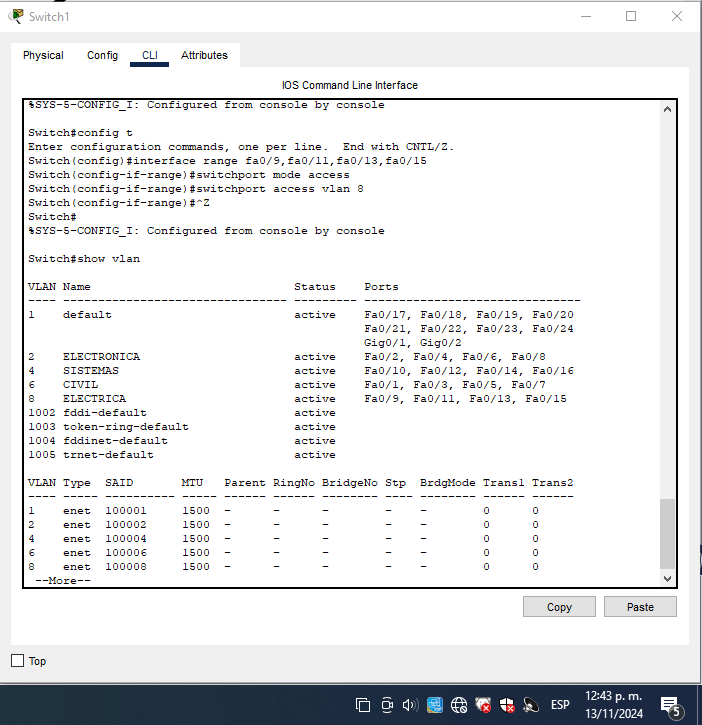
\includegraphics[width=0.6\textwidth]{img/cisco_vlan_PC1.png}
            \caption{Configuración de todos los VLAN's en el Switch del simulador Cisco Packet Tracer}
            \label{fig:cisco_vlan_PC1}
        \end{figure}

        Para probar la configuración de las VLAN's, se ingresó a la página web de cada servidor desde las PC's asignadas a cada departamento. La dirección IP de cada servidor se muestra en la tabla~\ref{tab:IPs}.

        \begin{table}[H]
            \begin{center}
                \begin{tabular}{ c | c | c | c }
                    \textbf{VLAN perteneciente} & \textbf{Servidor} & \textbf{Dirección IP} & \textbf{Máscara de subred}\\ \hline
                    2 & Electrónica & 1.0.0.100 & 255.0.0.0\\
                    4 & Sistemas & 10.0.0.100 & 255.0.0.0\\
                    6 & Civil & 172.16.0.100 & 255.255.0.0\\
                    8 & Eléctrica & 192.168.6.100 & 255.255.255.0\\
                \end{tabular}
                \caption{Direcciones IP de los servidores}
                \label{tab:IPs}
                \end{center}
        \end{table}

        Desde la PC E1, el cual pertenece al departamento de Electrónica, se ingresó a la página web del servidor, cuya dirección IP es \texttt{1.0.0.100} como se muestra en la figura~\ref{fig:servidor_electronica_PC1}.

        \begin{figure}[H]
            \centering
            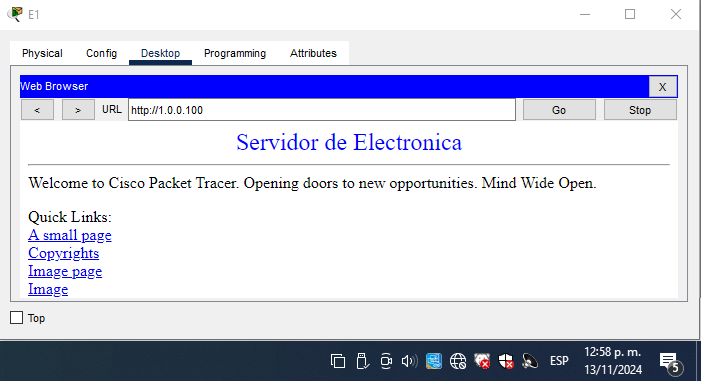
\includegraphics[width=0.7\textwidth]{img/servidor_electronica_PC1.png}
            \caption{Página web del servidor de Electrónica}
            \label{fig:servidor_electronica_PC1}
        \end{figure}

        Desde la PC S1, el cual pertenece al departamento de Sistemas, se ingresó a la página web del servidor, cuya dirección IP es \texttt{10.0.0.100} como se muestra en la figura~\ref{fig:servidor_sistemas_PC1}.

        \begin{figure}[H]
            \centering
            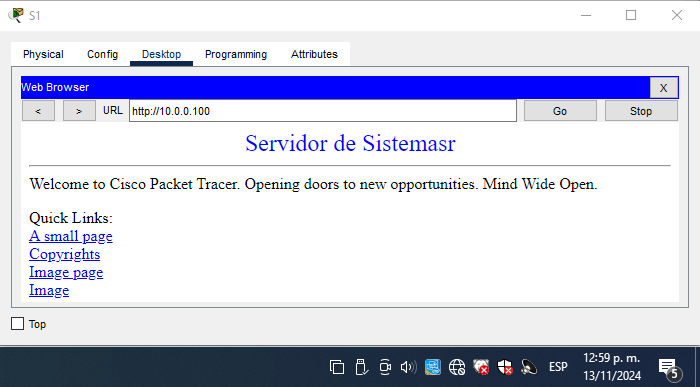
\includegraphics[width=0.7\textwidth]{img/servidor_sistemaPC1.png}
            \caption{Página web del servidor de Sistemas}
            \label{fig:servidor_sistemas_PC1}
        \end{figure}

        Desde la PC C1, el cual pertenece al departamento de Civil, se ingresó a la página web del servidor, cuya dirección IP es \texttt{172.16.0.100} como se muestra en la figura~\ref{fig:servidor_civil_PC1}.

        \begin{figure}[H]
            \centering
            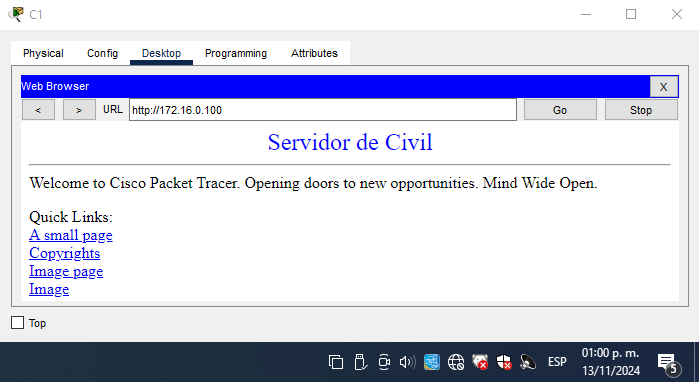
\includegraphics[width=0.7\textwidth]{img/servidor_civil_PC1.png}
            \caption{Página web del servidor de Civil}
            \label{fig:servidor_civil_PC1}
        \end{figure}

        Desde la PC1, el cual pertenece al departamento de Eléctrica, se ingresó a la página web del servidor, cuya dirección IP es \texttt{192.168.6.100} como se muestra en la figura~\ref{fig:servidor_electrica_PC1}.

        \begin{figure}[H]
            \centering
            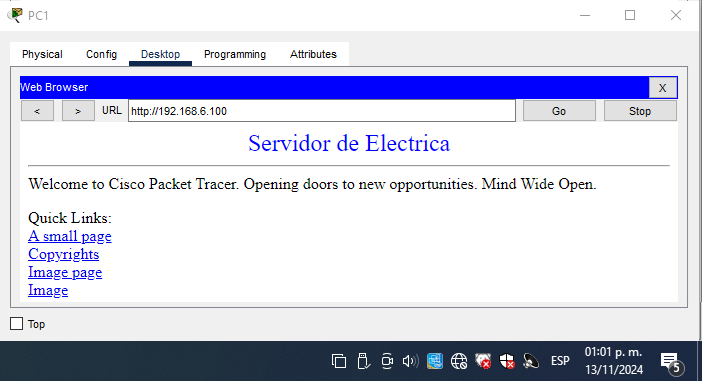
\includegraphics[width=0.7\textwidth]{img/servidor_electrica_PC1.png}
            \caption{Página web del servidor de Eléctrica}
            \label{fig:servidor_electrica_PC1}
        \end{figure}

        Cada PC se conectó a la página web del servidor correspondiente a su departamento, lo que indica que la configuración de las VLAN's fue exitosa.

    \subsection{Configuración de las VLAN's en Cisco Packet Tracer PC2}
        Para comenzar la configuración, en el simulador agregaremos un switch, 4 servidores y 12 PC's. Luego, conectaremos los dispositivos de acuerdo con el puerto asignado en la tabla 1, según la VLAN que se deba asignar. En la figura 7 se puede observar la configuración en el simulador.

        \begin{figure}[H]
            \centering
            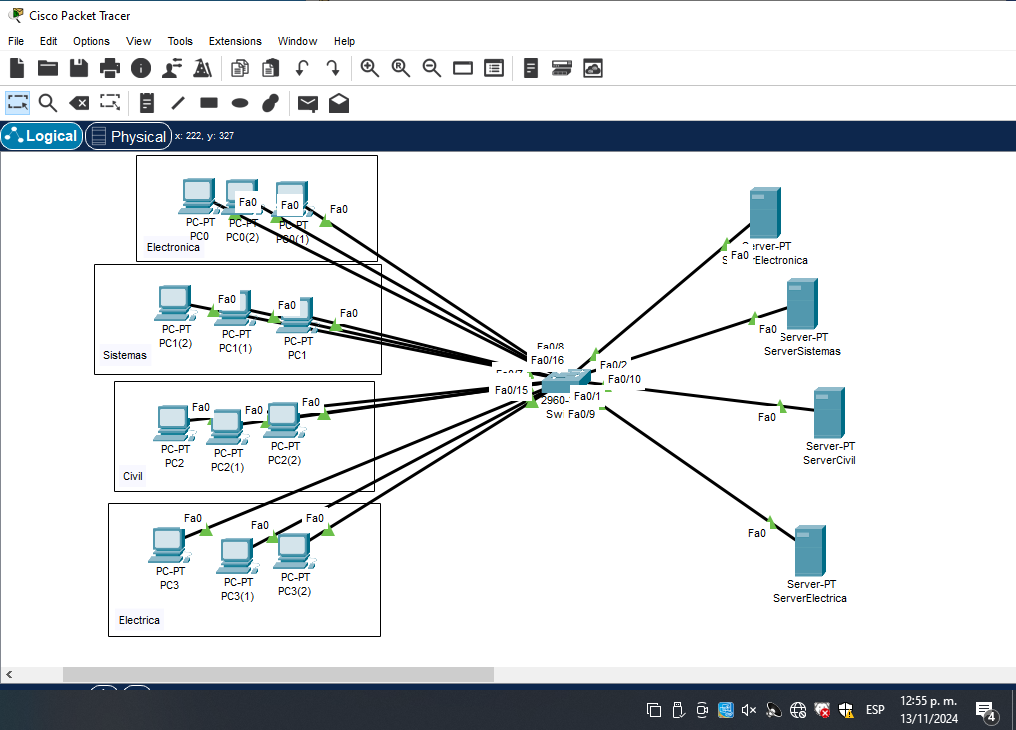
\includegraphics[width=0.7\textwidth]{img/Grafica.PNG}
            \caption{Configuración en el simulador de la PC2}
            \label{fig:Grafica}
        \end{figure}

        Para la configuración del Switch utilizaremos las líneas de código 1, 2, 3, 4 que se muestran en el documento para la creación de las VLAN's.

        En la figura 8 se muestra la configuración de todos los VLAN's en el Switch del simulador Cisco Packet Tracer.

        \begin{figure}[H]
            \centering
            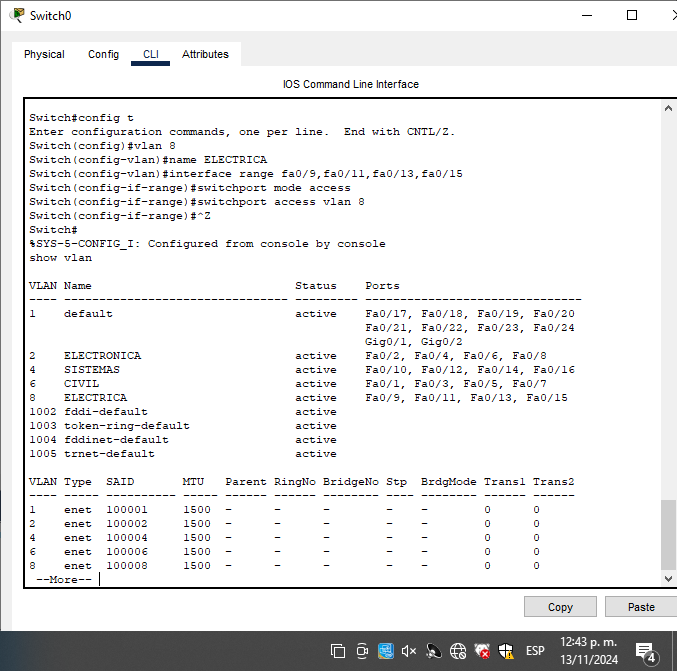
\includegraphics[width=0.7\textwidth]{img/Captura.PNG}
            \caption{Configuración de todos los VLAN's en Switch en el simulador de la PC2}
            \label{fig:Captura}
        \end{figure}

        Para el siguiente paso conectaremos las PC's con el servidor de forma que nos aparezca un mensaje personalizado.

        Desde la PC E1, el cual pertenece al departamento de Electrónica, se ingresó a la página web del servidor, cuya dirección IP es \texttt{1.0.0.10} como se muestra en la figura~\ref{fig:servidorElectronica}.


        \begin{figure}[H]
            \centering
            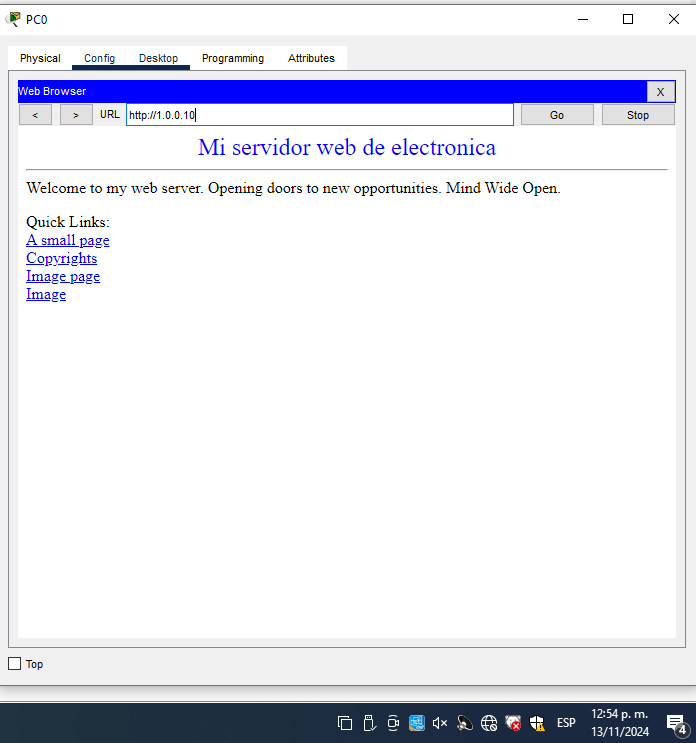
\includegraphics[width=0.7\textwidth]{img/serverElectronica.PNG}
            \caption{Página web del servidor de Electrónica}
            \label{fig:servidorElectronica}
        \end{figure}

        Desde la PC S1, el cual pertenece al departamento de Sistemas, se ingresó a la página web del servidor, cuya dirección IP es \texttt{10.0.0.10} como se muestra en la figura~\ref{fig:servidorSistemas}.

        \begin{figure}[H]
            \centering
            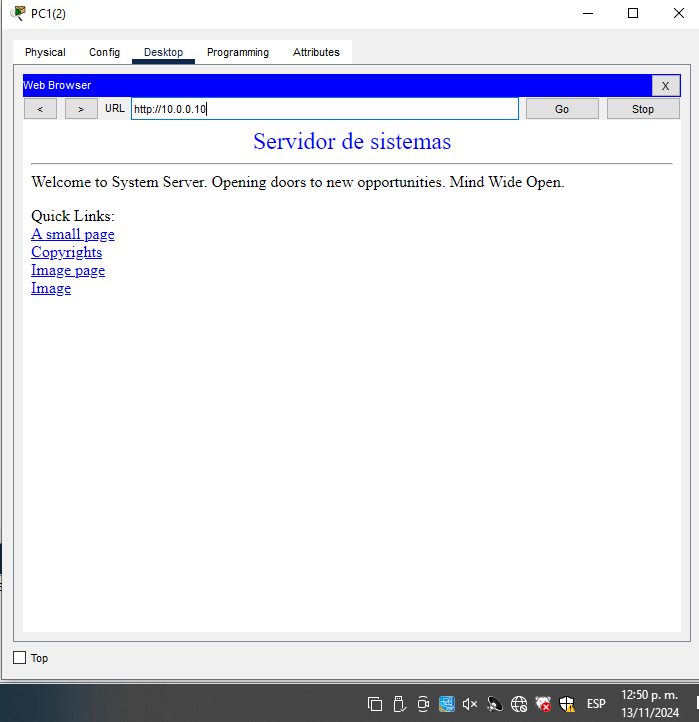
\includegraphics[width=0.7\textwidth]{img/Servidor de sistemas.PNG}
            \caption{Página web del servidor de Sistemas}
            \label{fig:servidorSistemas}
        \end{figure}

        Desde la PC C1, el cual pertenece al departamento de Civil, se ingresó a la página web del servidor, cuya dirección IP es \texttt{172.16.0.10} como se muestra en la figura~\ref{fig:servidorCivil}.

        \begin{figure}[H]
            \centering
            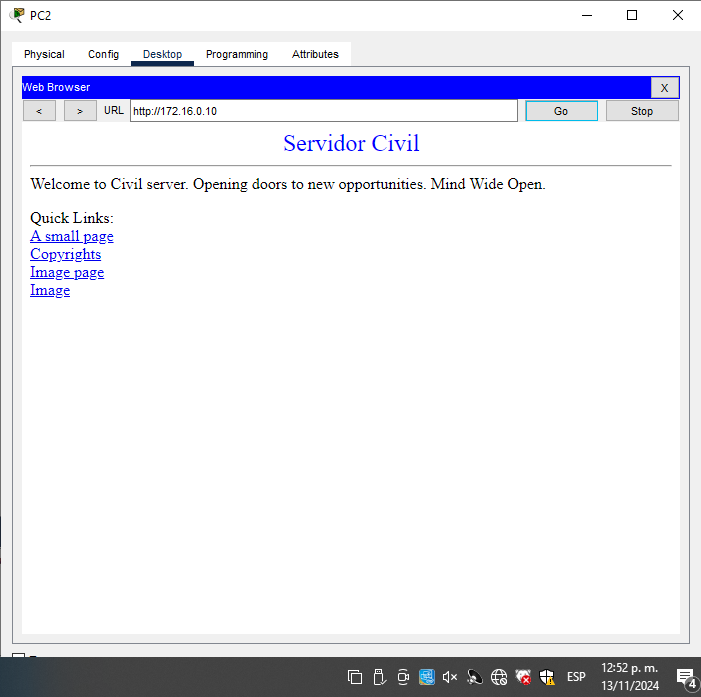
\includegraphics[width=0.7\textwidth]{img/ServerCivil.PNG}
            \caption{Página web del servidor de Civil}
            \label{fig:servidorCivil}
        \end{figure}

        Desde la PC1, el cual pertenece al departamento de Eléctrica, se ingresó a la página web del servidor, cuya dirección IP es \texttt{192.168.6.10} como se muestra en la figura~\ref{fig:servidorElectrica}.

        \begin{figure}[H]
            \centering
            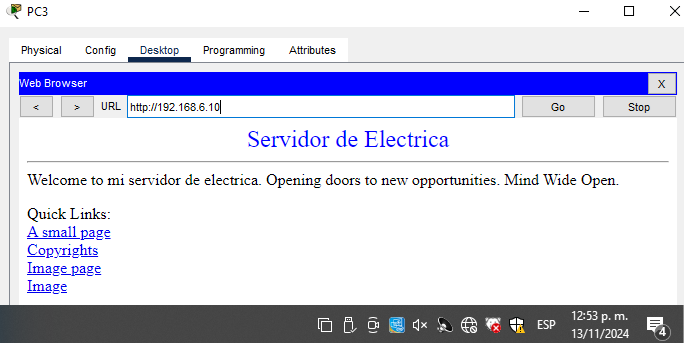
\includegraphics[width=0.7\textwidth]{img/serverElectrica.PNG}
            \caption{Página web del servidor de Eléctrica}
            \label{fig:servidorElectrica}
        \end{figure}

        Cada PC se conectó a la página web del servidor correspondiente a su departamento, lo que indica que la configuración de las VLAN's fue exitosa.



    \subsection{Configuración de las VLAN's en el Switch}
        Para comenzar, debemos conectar un extremo de un cable recto al puerto de consola del switch y el otro extremo al puerto serie del PC. Posteriormente, abrimos el programa de HyperTerminal y configuramos el puerto serie con los siguientes parámetros: 9600 baudios, 8 bits de datos, 1 bit de parada, sin bits de paridad y sin control de flujo, como se muestra en la figura~\ref{fig:HyperTerminal}.

        \begin{figure}[H]
            \centering
            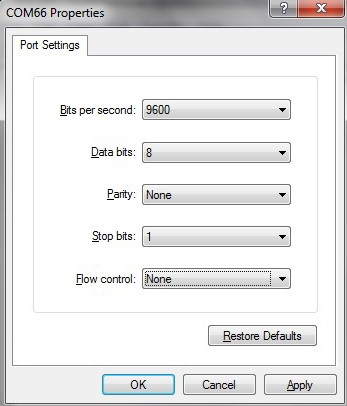
\includegraphics[width=0.7\textwidth]{img/HyperTerminal.jpg}
            \caption{Configuración de HyperTerminal}
            \label{fig:HyperTerminal}
        \end{figure}

        Posteriormente, encendemos el switch y presionamos la tecla Enter para acceder al modo de configuración. Luego, ingresamos el comando \texttt{enable} para acceder al modo privilegiado y el comando \texttt{configure t} para acceder al modo de configuración global. A continuación, creamos las VLAN's con los comandos mostrados en el código~\ref{lst:vlansSwitch}.

        \begin{lstlisting}[language=bash, caption={Creación de las VLAN's en el Switch},label={lst:vlansSwitch}]
            Switch> enable
            Switch# configure terminal
            Switch(config)# vlan 2
            Switch(config-vlan)# name ELECTRONICA
            Switch(config)# vlan 4
            Switch(config-vlan)# name SISTEMAS
            Switch(config)# vlan 6
            Switch(config-vlan)# name CIVIL
            Switch(config)# vlan 8
            Switch(config-vlan)# name ELECTRICA
        \end{lstlisting}

        Luego, asignamos los puertos a las VLAN's creadas anteriormente con los siguientes comandos, como se puede ver en el código~\ref{lst:asignacionPuertos}.

        \begin{lstlisting}[language=bash, caption={Asignación de puertos a las VLAN's en el Switch},label={lst:asignacionPuertos}]
            Switch(config)# interface range fa0/2, fa0/4, fa0/6, fa0/8
            Switch(config-if-range)# switchport mode access
            Switch(config-if-range)# switchport access vlan 2
            Switch(config)# interface range fa0/10, fa0/12, fa0/14, fa0/16
            Switch(config-if-range)# switchport mode access
            Switch(config-if-range)# switchport access vlan 4
            Switch(config)# interface range fa0/1, fa0/3, fa0/5, fa0/7
            Switch(config-if-range)# switchport mode access
            Switch(config-if-range)# switchport access vlan 6
            Switch(config)# interface range fa0/9, fa0/11, fa0/13, fa0/15
            Switch(config-if-range)# switchport mode access
            Switch(config-if-range)# switchport access vlan 8
        \end{lstlisting}

        Finalmente, verificamos la configuración de las VLAN's con el comando \texttt{show vlan} como se muestra en la figura~\ref{fig:vlansSwitch}. Y podemos observar que los puertos están asignados a las VLAN's correspondientes.

        \begin{figure}[H]
            \centering
            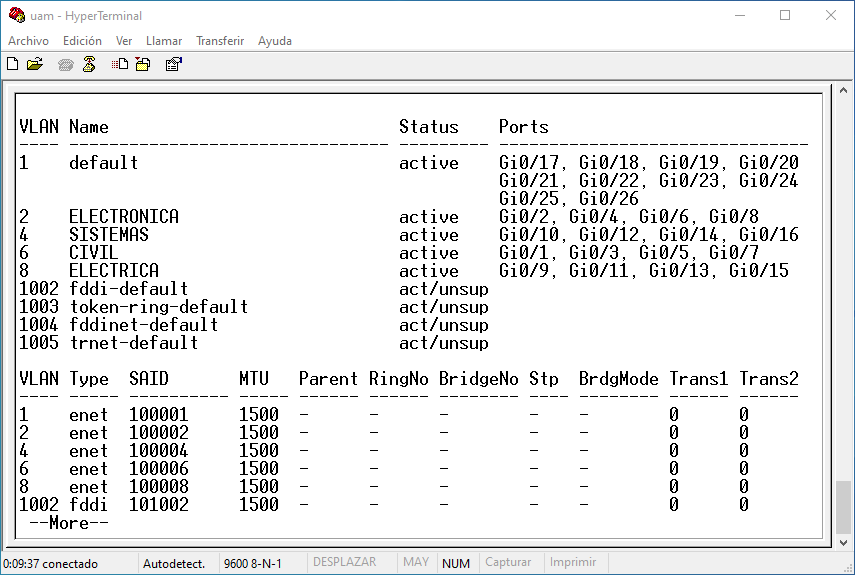
\includegraphics[width=0.7\textwidth]{img/vlansSwitch.png}
            \caption{VLAN's creadas en el Switch}
            \label{fig:vlansSwitch}
        \end{figure}

        Para comenzar, la PC1 y la PC2 se conectó a un puerto del switch el cual está asignada la VLAN por default, la PC1 se conectó al puerto 20 y la PC2 al puerto 21. Posteriormente, se asignó manualmente la dirección IP  a la PC1 el cual es \texttt{192.168.1.13/24} y a la PC2 el cual es \texttt{192.168.1.14/24}. Luego, se realizó un ping entre ambas PC's, como se muestra en la figura~\ref{fig:ping_default}. Esto se realizó para verificar la conectividad entre las PC's y el switch.

        \begin{figure}[H]
            \centering
            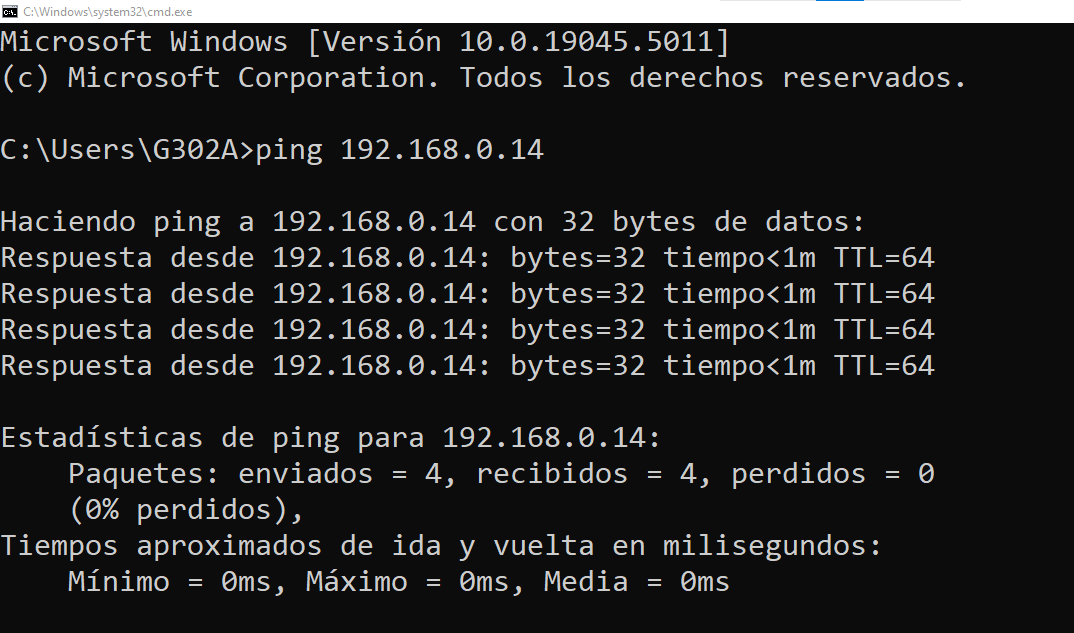
\includegraphics[width=0.7\textwidth]{img/ping_default.png}
            \caption{VLAN default en el Switch}
            \label{fig:ping_default}
        \end{figure}

        Posteriormente, se verificó el funcionamiento de la VLAN 2, para esto, la PC1 se conectó al puerto 2 del switch, y se le asignó manualmente la dirección IP \texttt{1.0.0.13/8}. Asimismo, la PC2 se conectó al puerto 4 del switch, y se le asignó manualmente la dirección IP \texttt{1.0.0.14/8}. Se realizó un ping entre ambas PC's, como se muestra en la figura~\ref{fig:ping_vlan2}.

        \begin{figure}[H]
            \centering
            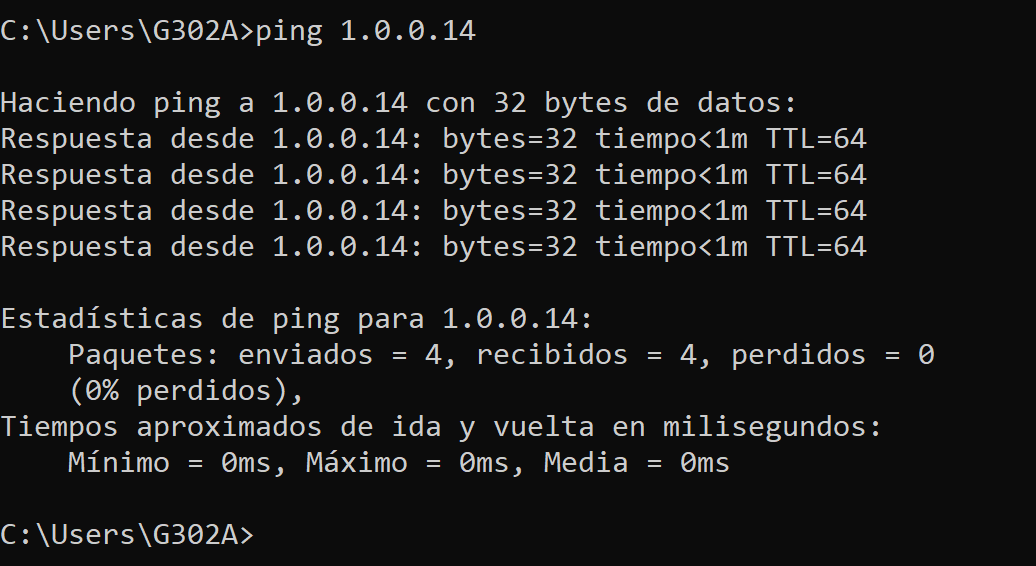
\includegraphics[width=0.7\textwidth]{img/ping_vlan2.png}
            \caption{VLAN 2 en el Switch}
            \label{fig:ping_vlan2}
        \end{figure}

        Para verificar el funcionamiento de la VLAN 4, la PC1 se conectó al puerto 10 del switch, y se le asignó manualmente la dirección IP \texttt{10.0.0.13/8}. Asimismo, la PC2 se conectó al puerto 12 del switch, y se le asignó manualmente la dirección IP \texttt{10.0.0.14/8}. Se realizó un ping entre ambas PC's, como se muestra en la figura~\ref{fig:ping_vlan4}.

        \begin{figure}[H]
            \centering
            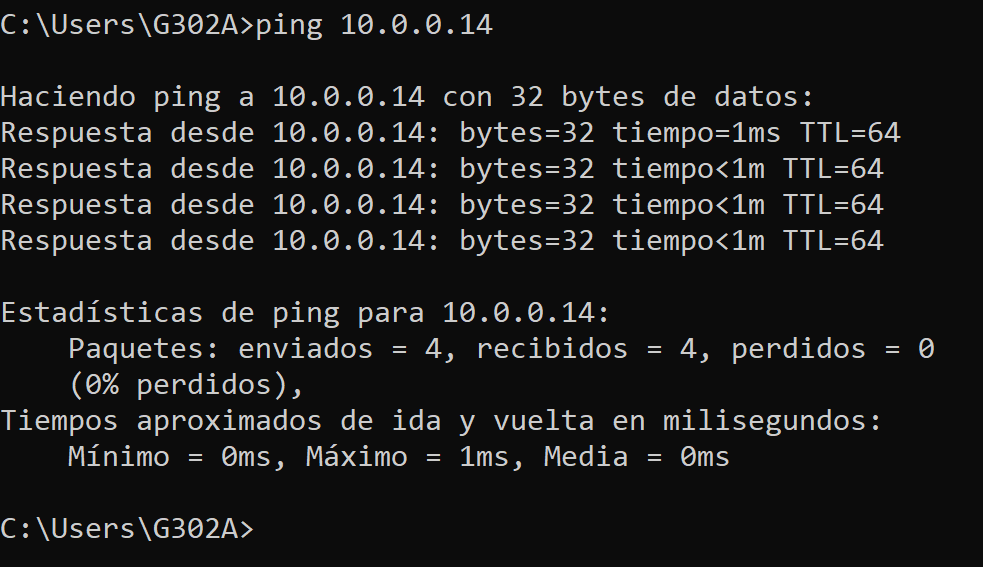
\includegraphics[width=0.7\textwidth]{img/ping_vlan4.png}
            \caption{VLAN 4 en el Switch}
            \label{fig:ping_vlan4}
        \end{figure}

        Para verificar el funcionamiento de la VLAN 6, la PC1 se conectó al puerto 1 del switch, y se le asignó la dirección IP \texttt{172.16.0.13/16}. Asimismo, la PC2 se conectó al puerto 3 del switch, y se le asignó manualmente la dirección IP \texttt{172.16.0.14/16}. Se realizó un ping entre ambas PC's, como se muestra en la figura~\ref{fig:ping_vlan6}.

        \begin{figure}[H]
            \centering
            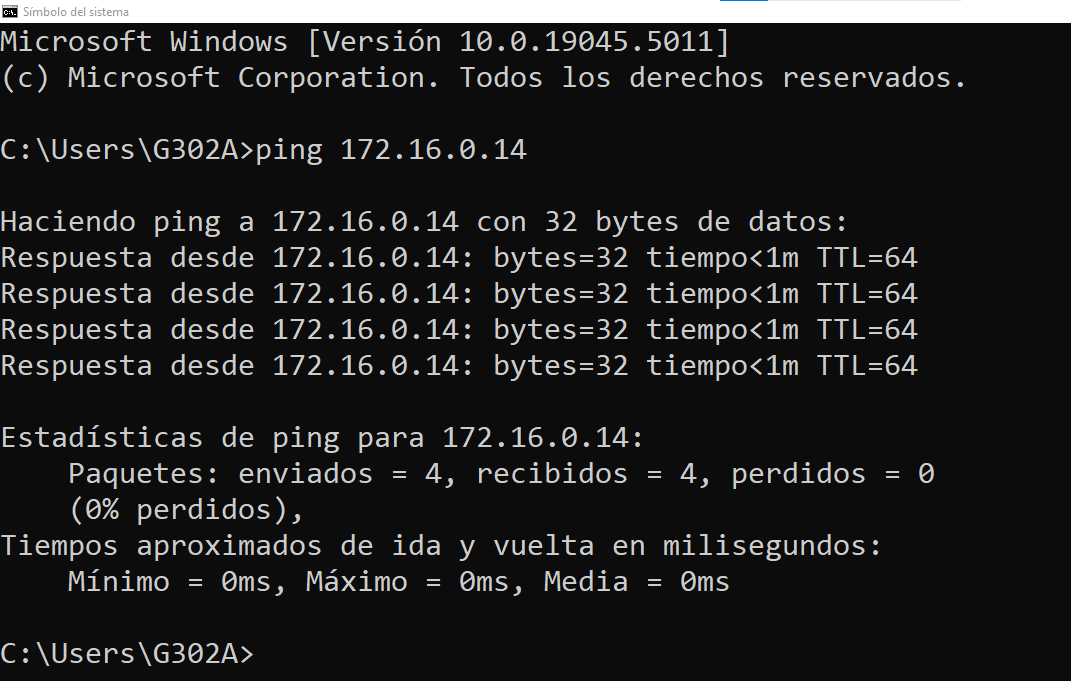
\includegraphics[width=0.7\textwidth]{img/ping_vlan6.png}
            \caption{VLAN 6 en el Switch}
            \label{fig:ping_vlan6}
        \end{figure}

        Finalmente, para verificar el funcionamiento de la VLAN 8, la PC1 se conectó al puerto 9 del switch, y se le asignó manualmente la dirección IP \texttt{192.168.6.13/24}. Asimismo, la PC2 se conectó al puerto 11 del switch, y se le asignó manualmente la dirección IP \texttt{192.168.6.14/24}. Se realizó un ping entre ambas PC's, como se muestra en la figura~\ref{fig:ping_vlan8}.

        \begin{figure}[H]
            \centering
            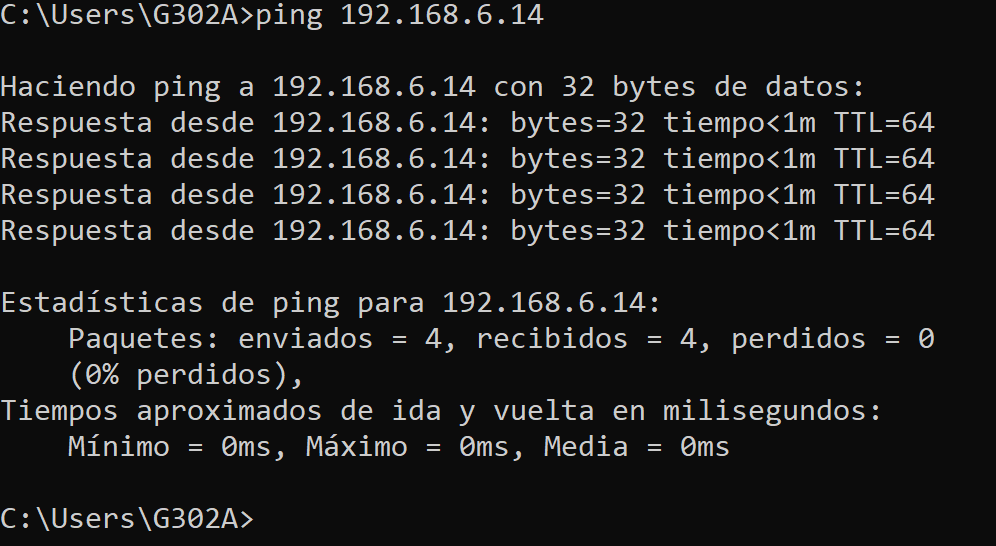
\includegraphics[width=0.7\textwidth]{img/ping_vlan8.png}
            \caption{VLAN 8 en el Switch}
            \label{fig:ping_vlan8}
        \end{figure}

\section{Conclusiones}
    \begin{itemize}
        \item Luis Ángel Cruz Díaz - 2183038433 \\
        Esta práctica mostró como las VLAN's permiten segmentar una red física en múltiples redes lógicas, lo que ayuda al no permitir que los dispositivos de una VLAN se comuniquen con los de otra VLAN. Esto es util en entornos corporativos donde se necesita separar los departamentos para mejorar la seguridad y la administración de la red.
        \item Diego Alexis Moreno Valero - 2243900185 \\
        En el desarrollo de esta práctica se logró aplicar los conceptos fundamentales sobre Redes de Área Local Virtual (VLAN), fortaleciendo habilidades en el diseño y configuración de redes segmentadas. A través de la herramienta Cisco Packet Tracer, configuramos VLAN's para distintos departamentos. Además, se asignaron dispositivos según las necesidades de cada grupo y se realizaron pruebas de conectividad que verificaron el éxito de la configuración.
    \end{itemize}
    
% --- Para agregar un apéndice
%\newpage
%\appendix
%\appendixpage
%\addappheadtotoc
%\section{Nombre del apéndice}